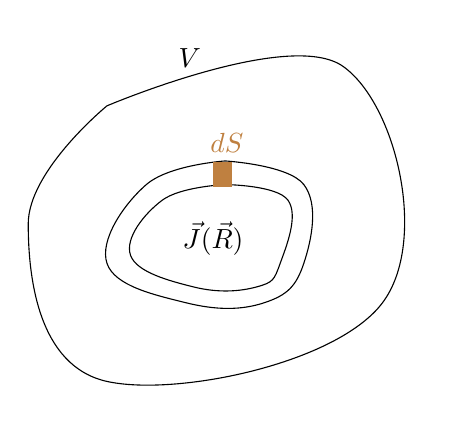
\begin{tikzpicture}
\draw  plot[smooth, tension=.7] coordinates {(0,0.8) (-1,0.5) (-1.5,-0.5) (-0.5,-1) (0.5,-1) (1,-0.5) (1,0.5) (0,0.8)};
\draw  plot[smooth, tension=.7] coordinates {(0,0.5) (-0.8,0.3) (-1.2,-0.4) (-0.4,-0.8) (0.4,-0.8) (0.7,-0.5) (0.8,0.3) (0,0.5)};
\draw  plot[smooth, tension=.7] coordinates {(-1.5,1.5) (-2.5,0) (-1.5,-2) (2,-1) (1.5,2) (-1.5,1.5)};
\draw [fill, brown]  (-0.1425,0.7829) rectangle (0.0787,0.4786);
\node at (0.0234,1.0318) [brown] {$dS$};
\node at (-0.1518,-0.1853) {$\vec{J}(\vec{R})$};
\node at (-0.4468,2.1014) {$V$};
\end{tikzpicture}